\chapter{Технологический раздел}
\label{cha:impl}

В данном разделе будут составлены требования к программному обеспечению, выбраны средства реализации и определены тестовые данные.

\section{Требования к программному обеспечению}
Требования к вводу:
\begin{itemize}
    \item $n \in \mathbb{N}$ - размер перемножаемых квадратных матриц;
    \item $n \cdot{} n$ действительных чисел, разделенных символами-разделителями (пробел, перенос строки, табуляция и т.п.) - элементы первой матрицы, перечисленные построчно;
    \item $n \cdot{} n$ действительных чисел, разделенных символами-разделителями - элементы второй матрицы, перечисленные построчно.
\end{itemize}
Требования к выводу:
\begin{itemize}
    \item результат умножения матриц.
\end{itemize}

\section{Средства реализации}
Для реализации программы вычисления редакционного расстояния мной был выбран язык программирования C++. В рамках текущей задачи данный язык программирования имеет ряд существенных преимуществ:
\begin{itemize}
    \item Статическая типизация;
    \item Близость к низкоуровневому C при наличии многих возможностей высокоуровненных языков;
    \item Встроенная библиотека std::chrono, позволяющая измерять процессорное время \cite{chrono}.
    \item Встроенная библиотека std::thread, содержащая класс нативных потоков \cite{thread}.
\end{itemize}

\section{Листинги кода}

В листингах \ref{lst:m1}, \ref{lst:m2}, \ref{lst:m3} приведен текст структуры и методов, описывающих умножение матриц по алгоритму Винограда.

\begin{lstlisting}[caption={Алгоритм Винограда, ч. 1}, label=lst:m1]
struct MatrixMul
{
    MatrixMul(double **m1, double **m2, size_t n, size_t m, size_t r);

    double **matrix1;
    double **matrix2;

    size_t n;
    size_t m;
    size_t r;

    double *mulh;
    double *mulv;
    double **res;

    void allocateMemory();
    void calculateMulh();
    void calculateMulv();
    void calculatePart1();
    void calculatePart2();
    void calculateUneven();
};
\end{lstlisting}

\begin{lstlisting}[caption={Алгоритм Винограда, ч. 2}, label=lst:m2]
MatrixMul::MatrixMul(double **m1, double **m2,
                     size_t n, size_t m, size_t r) :
    matrix1(m1), matrix2(m2), n(n), m(m), r(r),
    mulh(nullptr), mulv(nullptr), res(nullptr)
{
}

void MatrixMul::allocateMemory()
{
    mulh = new double[n];
    mulv = new double[m];

    res = Util::createMatrix<double>(n, m);
}

void MatrixMul::calculateMulh()
{
    double temp;
    size_t r_div_2 = r >> 1;

    for (size_t i = 0; i < n; i++)
    {
        temp = 0;

        for (size_t j = 0; j < r_div_2; j++)
        {
            temp += matrix1[i][j << 1] * matrix1[i][(j << 1) + 1];
        }

        mulh[i] = temp;
    }
}

void MatrixMul::calculateMulv()
{
    double temp;
    size_t r_div_2 = r >> 1;

    for (size_t j = 0; j < m; j++)
    {
        temp = 0;

        for (size_t i = 0; i < r_div_2; i++)
        {
            temp += matrix2[i << 1][j] * matrix2[(i << 1) + 1][j];
        }

        mulv[j] = temp;
    }
}
\end{lstlisting}

\begin{lstlisting}[caption={Алгоритм Винограда, ч. 3}, label=lst:m3]
void MatrixMul::calculatePart1()
{
    double temp;

    size_t r_div_2 = r >> 1;
    size_t n_div_2 = n >> 1;

    for (size_t i = 0; i < n_div_2; i++)
    {
        for (size_t j = 0; j < m; j++)
        {
            temp = -(mulh[i] + mulv[j]);

            for (size_t k = 0; k < r_div_2; k++)
            {
                temp += (matrix1[i][k << 1] + matrix2[(k << 1) + 1][j]) *
                        (matrix1[i][(k << 1) + 1] + matrix2[k << 1][j]);
            }

            res[i][j] = temp;
        }
    }
}

void MatrixMul::calculatePart2()
{
    double temp;

    size_t r_div_2 = r >> 1;
    size_t n_div_2 = n >> 1;

    for (size_t i = n_div_2; i < n; i++)
    {
        for (size_t j = 0; j < m; j++)
        {
            temp = -(mulh[i] + mulv[j]);

            for (size_t k = 0; k < r_div_2; k++)
            {
                temp += (matrix1[i][k << 1] + matrix2[(k << 1) + 1][j]) *
                        (matrix1[i][(k << 1) + 1] + matrix2[k << 1][j]);
            }

            res[i][j] = temp;
        }
    }
}

void MatrixMul::calculateUneven()
{
    if (r & 1)
    {
        for (size_t i = 0; i < n; i++)
            for (size_t j = 0; j < m; j++)
                res[i][j] += matrix1[i][r - 1] * matrix2[r - 1][j];
    }

    delete[] mulh;
    delete[] mulv;

    mulh = nullptr;
    mulv = nullptr;
}
\end{lstlisting}

В листингах \ref{lst:c1}, \ref{lst:c2} приведен текст структуры и методов, описывающих конвейер умножения матриц по алгоритму Винограда.

\begin{lstlisting}[caption={Конвейер перемножения матриц по алгоритму Винограда, ч. 1}, label=lst:c1]
class MatrixMulReader
{
public:
    virtual struct MatrixMul operator()() = 0;
    virtual operator bool() = 0;
};

class Conveyor
{
public:
    static
    void do1(MatrixMulReader *mmr)
    {
        while (*mmr)
        {
            auto mm = (*mmr)();
            mm.allocateMemory();

            m12.lock();
            q12.push(mm);
            m12.unlock();
        }

        isP1Ended = true;
    }
    static
    void do2()
    {
        while (!q12.empty() || !isP1Ended)
        {
            if (!q12.empty())
            {
                m12.lock();
                struct MatrixMul mm = q12.front();;
                q12.pop();
                m12.unlock();

                mm.calculateMulh();

                m23.lock();
                q23.push(mm);
                m23.unlock();
            }
        }

        isP1Ended = false;
        isP2Ended = true;
    }
    static
    void do3()
    {
        while (!q23.empty() || !isP2Ended)
        {
            if (!q23.empty())
            {
                m23.lock();
                struct MatrixMul mm = q23.front();
                q23.pop();
                m23.unlock();

                mm.calculateMulv();

                m34.lock();
                q34.push(mm);
                m34.unlock();
            }
        }

        isP2Ended = false;
        isP3Ended = true;
    }
\end{lstlisting}

\begin{lstlisting}[caption={Конвейер перемножения матриц по алгоритму Винограда, ч. 2}, label=lst:c2]
    static
    void do4()
    {
        while (!q34.empty() || !isP3Ended)
        {
            if (!q34.empty())
            {
                m34.lock();
                struct MatrixMul mm = q34.front();
                q34.pop();
                m34.unlock();

                mm.calculatePart1();

                m45.lock();
                q45.push(mm);
                m45.unlock();
            }
        }

        isP3Ended = false;
        isP4Ended = true;
    }
    static
    void do5()
    {
        while (!q45.empty() || !isP4Ended)
        {
            if (!q45.empty())
            {
                m45.lock();
                struct MatrixMul mm = q45.front();
                q45.pop();
                m45.unlock();

                mm.calculatePart2();

                m56.lock();
                q56.push(mm);
                m56.unlock();
            }
        }

        isP4Ended = false;
        isP5Ended = true;
    }
    static
    void do6()
    {
        while (!q56.empty() || !isP5Ended)
        {
            if (!q56.empty())
            {
                m56.lock();
                struct MatrixMul mm = q56.front();
                q56.pop();
                m56.unlock();

                mm.calculateUneven();

                q67.push(mm);
            }
        }

        isP5Ended = false;
    }

    static std::queue<struct MatrixMul> q12;
    static std::queue<struct MatrixMul> q23;
    static std::queue<struct MatrixMul> q34;
    static std::queue<struct MatrixMul> q45;
    static std::queue<struct MatrixMul> q56;
    static std::queue<struct MatrixMul> q67;

    static std::mutex m12;
    static std::mutex m23;
    static std::mutex m34;
    static std::mutex m45;
    static std::mutex m56;
    static std::mutex m67;

    static bool isP1Ended;
    static bool isP2Ended;
    static bool isP3Ended;
    static bool isP4Ended;
    static bool isP5Ended;
    static bool isP6Ended;
    static bool isP7Ended;
};
\end{lstlisting}

\section{Примеры работы}

На рисунках \ref{img:ex1}-\ref{img:ex5} приведены примеры работы.

\begin{figure}[H]
    \centering
    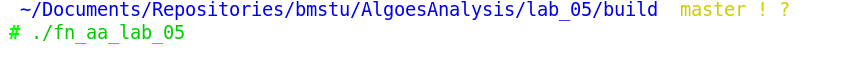
\includegraphics[scale=0.6]{./images/example1.png}
    \caption{Пустой ввод}
    \label{img:ex1}
\end{figure}

\begin{figure}[H]
    \centering
    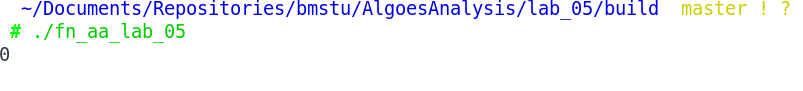
\includegraphics[scale=0.6]{./images/example2.png}
    \caption{Невозможная длина матрицы}
    \label{img:ex2}
\end{figure}

\begin{figure}[H]
    \centering
    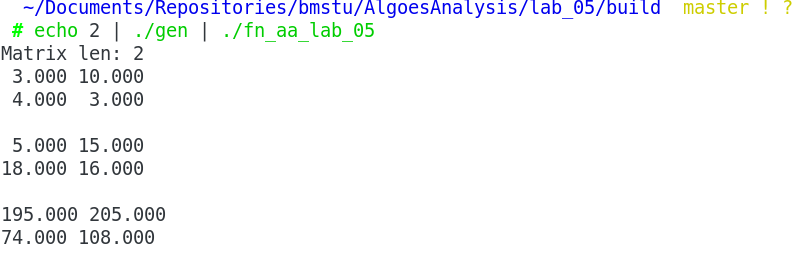
\includegraphics[scale=0.6]{./images/example3.png}
    \caption{Умножения квадратных матриц длины 2}
    \label{img:ex3}
\end{figure}

\begin{figure}[H]
    \centering
    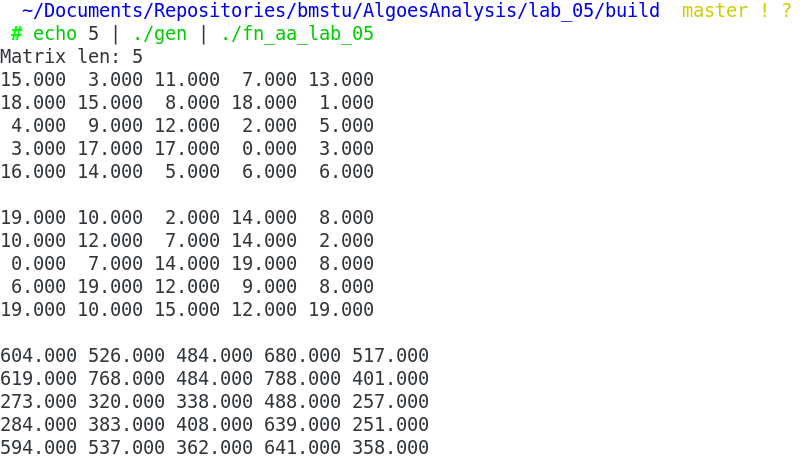
\includegraphics[scale=0.6]{./images/example4.png}
    \caption{Умножения квадратных матриц длины 5}
    \label{img:ex4}
\end{figure}

\begin{figure}[H]
    \centering
    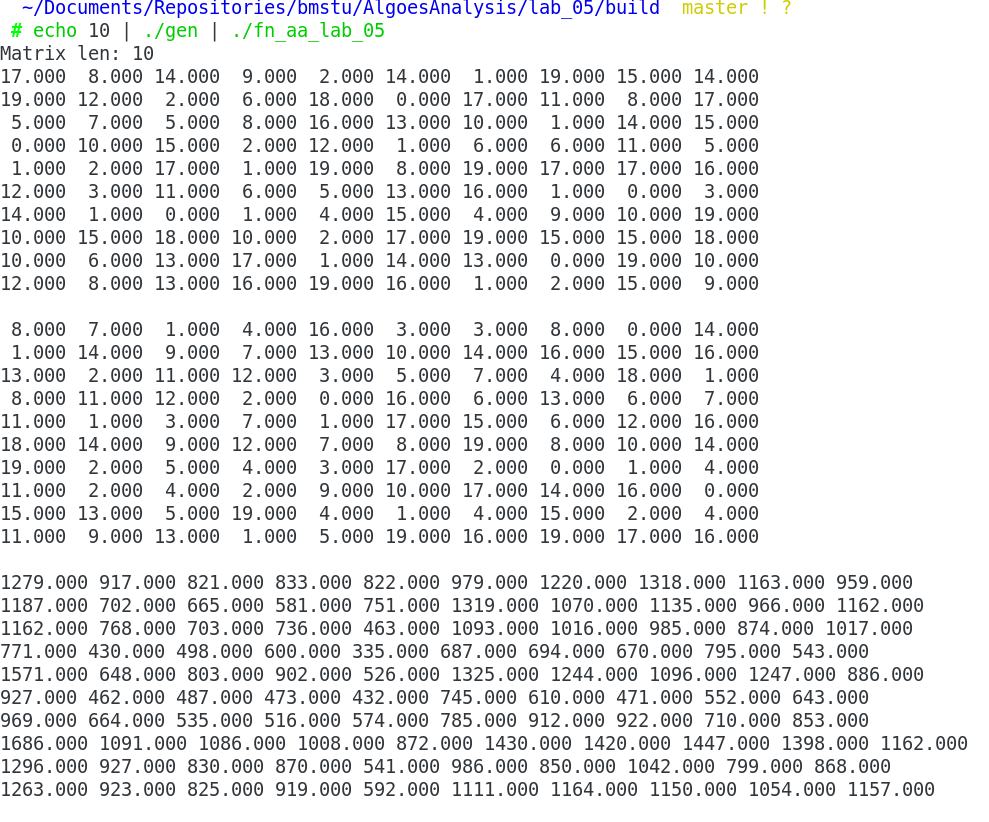
\includegraphics[scale=0.6]{./images/example5.png}
    \caption{Умножения квадратных матриц длины 10}
    \label{img:ex5}
\end{figure}

\section{Описание тестирования}

В таблице \ref{table:test} приведены тестовые данные.

\begin{table}[H]
    \caption{Тестовые данные}
    \label{table:test}
    \centering
    \begin{tabular}{|c|c|c|}
        \hline
        Первая матрица & Вторая матрица & Ожидаемый результат \\
        \hline
        1 2 & 1 2 & \ 7 10 \\
        3 4 & 3 4 & 15 22 \\
        \hline
        1 2 3 & 1 2 3 & \ 30\ \ 36\ \ 42 \\
        4 5 6 & 4 5 6 & \ 66\ \ 81\ \ 96 \\
        7 8 9 & 7 8 9 & 102 126 150 \\
        \hline
        1 0 0 & 1 2 3 & 1 2 3 \\
        0 1 0 & 4 5 6 & 4 5 6 \\
        0 0 1 & 7 8 9 & 7 8 9 \\
        \hline
    \end{tabular}
\end{table}

В таблицах \ref{table:wtest}, \ref{table:cwtest} приведены результаты тестирования. Все тесты были успешно пройдены.

\begin{table}[H]
    \caption{Результаты тестирования алгоритма Винограда}
    \label{table:wtest}
    \centering
    \begin{tabular}{|c|c|c|}
        \hline
        Первая матрица & Вторая матрица & Полученный результат \\
        \hline
        1 2 & 1 2 & \ 7 10 \\
        3 4 & 3 4 & 15 22 \\
        \hline
        1 2 3 & 1 2 3 & \ 30\ \ 36\ \ 42 \\
        4 5 6 & 4 5 6 & \ 66\ \ 81\ \ 96 \\
        7 8 9 & 7 8 9 & 102 126 150 \\
        \hline
        1 0 0 & 1 2 3 & 1 2 3 \\
        0 1 0 & 4 5 6 & 4 5 6 \\
        0 0 1 & 7 8 9 & 7 8 9 \\
        \hline
    \end{tabular}
\end{table}

\begin{table}[H]
    \caption{Результаты тестирования конвейерного алгоритма Винограда}
    \label{table:cwtest}
    \centering
    \begin{tabular}{|c|c|c|}
        \hline
        Первая матрица & Вторая матрица & Полученный результат \\
        \hline
        1 2 & 1 2 & \ 7 10 \\
        3 4 & 3 4 & 15 22 \\
        \hline
        1 2 3 & 1 2 3 & \ 30\ \ 36\ \ 42 \\
        4 5 6 & 4 5 6 & \ 66\ \ 81\ \ 96 \\
        7 8 9 & 7 8 9 & 102 126 150 \\
        \hline
        1 0 0 & 1 2 3 & 1 2 3 \\
        0 1 0 & 4 5 6 & 4 5 6 \\
        0 0 1 & 7 8 9 & 7 8 9 \\
        \hline
    \end{tabular}
\end{table}

\section{Вывод}
Для реализации программы были выбраны средства разработки: язык программирование C++, библиотеки std::chrono, std::thread, а так же подготовлены тестовые данные и успешно проведено тестирование.

